\chapter{Introduction}
\section{Motivation}
\hspace{10mm} Emergencies can happen at any time. From minor issues to severe trauma, It is essential that the response teams that come to help them are equipped with the necessary technology to save lives. There is an increasing demand for Emergency medical services (EMS). To respond to this growing demand, the EMS communities require adaptable and sustainable systems. First Responders or paramedics, as they are generally called in United States, provide rapid assessments and treatment of the sick while transporting them to a hospital for further evaluation. Considerable knowledge, skill, and suitable technology are required to provide quality ambulatory emergency medical services. High quality emergency medical services and paramedics are important part of any health care system. Paramedics often are first to arrive at the scene, and  are allowed to defibrillate, to intubate endotracheally, and to administer life-saving drugs (epinephrine endotracheally, glucose intravenously, etc.). They treat patients during transport in the ambulance. Many studies of pre-hospital services place greater emphasis on technology factors, human efficiency and continuous refinement of standards of practice.EMS providers are expected to render effective life-saving evaluation, intervention, stabilization and treatment that are consistent with existing standards and codes. Paramedics must be properly trained and equipped with suitable equipment, tools and systems to ensure that the highest quality of care, safety and reliability are attained before, during and after a medical emergency event \cite{EMS,EMS1,EMS2,EMS3}.

\hspace{10mm} These situation require responders to effectively care for patients with limited resources and medical infrastructure within the limited space inside the ambulance, often under intense time pressure. For years, emergency medical service providers conducted patient care by manually measuring vital signs, documenting assessments on paper, and communicating over handheld radios. The ability to automate these tasks could greatly relieve the workload for each responder, increase the quality and quantity of patient care, and more efficiently deliver patients to the hospital. 
Steady advances in wireless networking, medical sensors, and interoperability software create exciting possibilities for improving the way we provide emergency care. BlueBox is a project that explores and showcases how these advances in technology can be employed to assist patients and paramedics in times of emergency. 

\section{Related Work}

\subsection{Medical Information Tag}
\hspace{10mm}  Tia Gao et al., developed MiTag (Medical information tag) \ref{fig:miTag}, a cost effective 
wireless sensor platform that automatically track patients 
throughout each step of the emergency response process, from disaster 
scenes, to ambulances, to hospitals \cite{miTag}.
\begin{figure}[h]
	\centering
	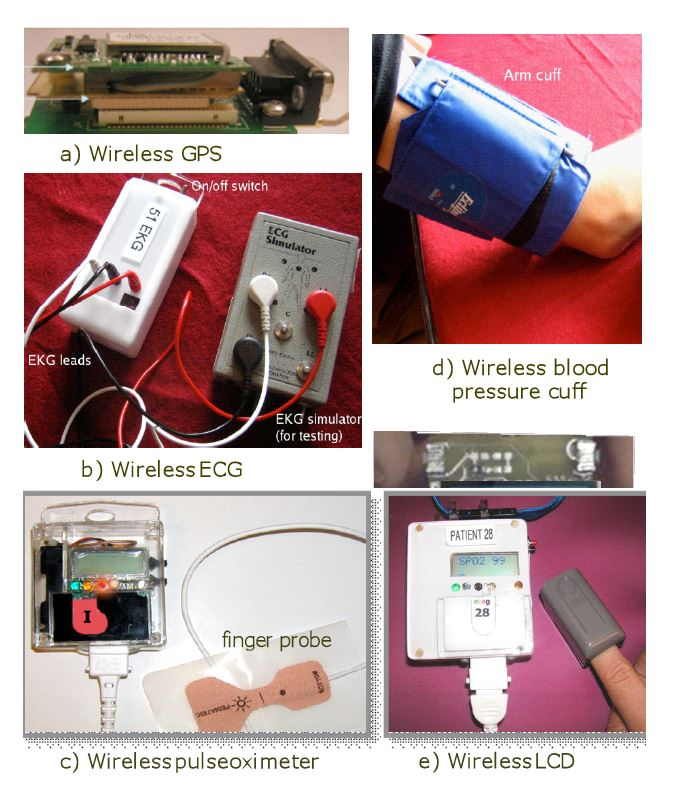
\includegraphics[scale = 0.6 ]{miTag.JPG}
	\caption{Medical Information Tag. Source \cite{miTag}\label{fig:miTag}}
\end{figure}
The miTags can increase 
the patient care capacity of responders in the field. The miTag  supports sensor add-ons – GPS, pulse oximetery, blood pressure and ECG. 
The miTag system is out-of-the-box operational and includes the following key technologies: 1) cost-effective sensor hardware, 2) 
self-organizing wireless network and 3) scalable server software 
that analyzes sensor data and delivers real-time updates to 
handheld devices and web portals. The drawback of this setup is its bulky size and uncomfortable usability. The miTag system has wireless blood pressure cuff with an additional 9V battery to power the cuff which makes it bulky. The miTag uses wireless sensors (ECG, GPS, Pulse oximeter), each of which has its own radio and battery, which makes each individual sensor bulky. This distributed nature of the system adds lot more work for paramedics to manage each one of them individually , which sometimes could be a pain. 
\subsection{Advanced Health
	and Disaster Aid Network (AID-N)}
\hspace{10mm}The Advanced Health and Disaster Aid Network (AID-N), developed by Tia Gao, Dan Greenspan et al., \cite{AID-N} at The Johns Hopkins University Applied Physics Laboratory, explores and showcases how these advances in technology can be employed to assist victims and responders in times of emergency. AID-N uses open-standard software and best-of-breed hardware to deliver a scalable, open, and reliable infrastructure that paves the way for the development of new capabilities and the extension of existing technologies. 
Wearable sensors designed by the CodeBlue project at Harvard University is used in AID-N. The AID-N system consists if a pulse oximeter sensor on patient's fingure that measures heart rate and blood oxygenation (SPO\textsubscript{2}) level of the patient.It uses Wearable sensors to sense and record vital signs into an electronic patient record database. The vitals are transmitted to a local base staion(a Tablet) that displays the vital in real time. Compared to MiTag this system requires very little setup as it has a single wearable setup. AID-N is integrated with pre-hospital patient care framework MICHAELS.Due to the chaotic nature of emergencies, AID-N system
faces the challenge of operating in situations that challenge instrumentation designed for use in
the controlled environment of a clinical situation. 


\section{Objective}
\hspace{10mm}The miTag and the AID-N systems presented above has challenges when it comes to the usability under a chaotic environment of emergency.Time is a critical resource during emergency and usability issue consumes this critical resource. Also the basic idea of building such devices is to help paramedics provide emergency care while maintaining record of the patients condition. But the above mentioned system does not provide space for paramedics to log about the patients response to their emergency treatment. BlueBox , the proposed system, addresses these issue.Collaborating with La BioMed we developed BlueBox (like Black Box device in a Aeroplanes) a low-cost, low-power wearable device that automates monitoring patient’s vitals and paramedic's log throughout each step of the response process.  The system provides a new paradigm to emergency response treatment by automating the patient monitoring process. The idea is to design an easy to use wearable hardware and integrate software solutions that records important  patient’s vitals and paramedic's logs in the database , which allows the doctors and physicians at the hospital to review . Access to this information could allow them to provide better care.

\hspace{10mm}BlueBox  platform support recording of variety of data including Electrocardiogram(ECG), body temperature, respiration pattern (through Chest movements monitoring and audio) , Environment temperature sensors, paramedic’s voice log about patient condition . BlueBox relieves the workload for paramedics by automating the task of data recording that helps improve quality of patient care and deliver patients to the hospital with a clear picture of patients condition from the time emergency. Our system accomplishes this through the following technologies:

\begin{itemize}
	\item Wearable sensors and electrodes to sense and record vital signs into an electronic storage.

	\item Microphones to record paramedic’s comments about the condition of the patient and synchronize with the vitals.
	
\end{itemize}

\section{Thesis Goals}
\hspace{10mm}The goal of this thesis is to build low power firmware for BlueBox which is designed to be wearable,battery operated easy-to-use . Wearable medical devices have strict size and weight constraints while having a functional and behavioural specifications that demands the system to have high performance and function for hours. Battery capacity is directly proportional to its size. Smaller the size and weight , lower the capacity of the battery\cite{}. Battery capacity is a huge bottleneck for these systems. So these systems requires an extensive power management strategies to be deployed in hardware and software level. This is a hardware-software cosynthesis problem.

Hence, in this thesis project, the goal can be stated as the following:

 \hspace{10mm}To build a low-power firmware for BlueBox system so that the device is able to acquire data at the required frequency and store the data in a local storage while functioning for atleast 3 hours. 
 
 The methods applied to accomplish the project can be elaborated as the following steps:
 \begin{itemize}
 	\item[$\bullet$] Understanding of the signal requirements and constraints. 
 	
 	\item[$\bullet$] Brainstorming on hardware and system design requirements to fulfill the behavioural specification and  mechanical constraints.
 	
 	\item[$\bullet$] Hardware software co-design to optimize the required resource and to implement the low-power data acquisition firmware.
 	
 	\item[$\bullet$] creating a simple interfacing software for data retrieval and data visualization on the PC
 	
 	\item[$\bullet$] testing, and conducting experiments with the firmware and the software,
 	along with the BlueBox system.
 \end{itemize}
 
\section{Thesis Organization}
The following chapters of this thesis report are organized as follows:
\begin{itemize}
	\item Chapter 2 gives a short overview of the BlueBox system. It also describes the significance and  requirements of the signal that needs to be recorded by the BlueBox system. This chapter also presents some design requirement confronted with some constraints
	
	\item Chapter 3 provides the final system overview and presents the hardware architecture. This chapter also talks about the important subsytems ,sensors and battery of the BlueBox system.
	
	\item  Chapter 4 explains the firmware architecture of the BlueBox system and describes its core functionalities. This chapter also talks about procedure for importing and visualizing the acquired data.
	
	\item Chapter 5 gives a background on general sources of power consumption and covers in details the power management techniques implemented in BlueBox firmware.
	
	\item Chapter 6 presents system setup, testing and verification of the BlueBox system. 
	
	\item
	Chapter 7 completes this report by giving the final conclusion and ideas for future enhancement of the device.
	
\end{itemize}
